Performing range query in a $K$D-tree needs to traverse the whole tree, but we can apply some pruning strategy to avoid useless searching for some nodes. We first present the \textbf{bounding box} of subtree in a $K$D-tree.

\begin{figure}[!htb]
     \centering
     \begin{subfigure}[b]{0.58\textwidth}
         \centering
         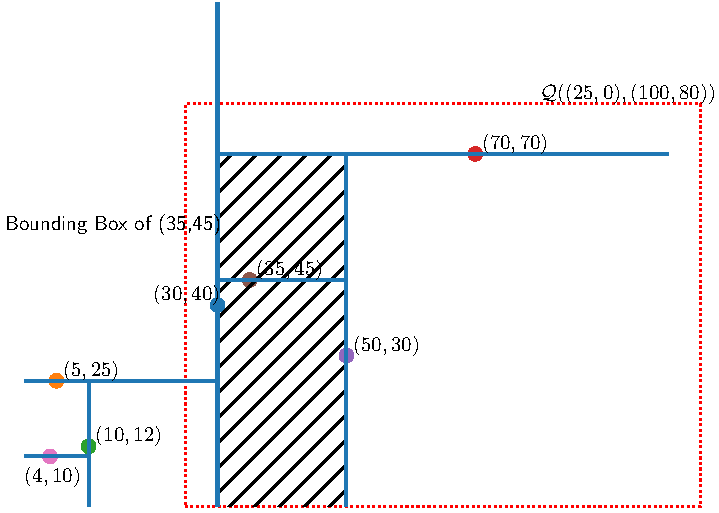
\includegraphics[width=\textwidth]{graphs/implementation/queries/range_query_kdtree}
         \caption{The $2$D space and the partition of $K$D-tree}
     \end{subfigure}
     \hfill
     \begin{subfigure}[b]{0.40\textwidth}
         \centering
         \begin{tikzpicture}
\tikzstyle{bplus}=[rectangle split, rectangle split horizontal,rectangle split ignore empty parts,draw]
\tikzstyle{every node}=[bplus]
\tikzstyle{level 1}=[sibling distance=30mm]
\tikzstyle{level 2}=[sibling distance=15mm]
\node {(30,40)} [->]
  child {node {(5,25)}
    child {node {(10,12)}
    	child {node {(4,10)}}
    	child[missing]{}
    }
    child[missing]{}    
  } 
  child {node {(70,70)}
    child {node {(50,30)}
    	child {node {(35,45)}}
    	child[missing]{}
    }
    child[missing]{}
  }
;\end{tikzpicture}
         \caption{The tree structure of the $K$D-tree}
     \end{subfigure}
        \caption{An example of $K$D-Tree}
        \label{fig:kdtree-rangequery}
\end{figure}

\noindent
\textbf{Bounding Box}

\noindent
When we are traversing the $K$D-tree along the way, we are assured that a node is bounded in a rectangle region. Assume that a node \texttt{t} has $k$ ancestors, then the node \texttt{t} is bounded in a rectangle in the following way: 

\begin{enumerate}
	\item We traverse from the root node whose coordinate is $(x_r, y_r)$. If we go to the right subtree, then the node \texttt{t} is bounded in the right side of the root node. That means, the right subtree of the root node is bounded in a rectangle region determined by the lower bound $\boldsymbol{l}=(x_r, 0)$\footnote{For simplicity and clarity, we assume our keys are starting from $(0,0)$ and are positive in both dimensions} and the upper bound $\boldsymbol{u}=(\infty, \infty)$. Similarly, we can determine the bounds of the left subtree as $\boldsymbol{l}=(0, 0)$ and $\boldsymbol{u}=(x_r, 0)$. We call the bounding box at this level as $B_0^r$ and $B_0^l$ for the right subtree and left subtree respectively.
	\item We then traverse into the next level and determine the bounding box $B_1^r$ and $B_1^l$ of the subtrees rooted at the root's child node. At this time, we will need to switch the axis into the $y$-axis. If the child node is in the left subtree of the root node, the final bounding box is the intersection between the bounding box at this level and the bounding box of left subtree at the root level, i.e. $B_0^l\cap B_1^r$ and $B_0^l\cap B_1^l$. Similarly, if the child node is in the right subtree of the root node, the final bounding box are $B_0^r\cap B_1^r$ and $B_0^r\cap B_1^l$.
	\item We traverse until the left node and determine the bounding box of each subtree and save this property into the root node of each subtree.
\end{enumerate}

\begin{mscexample}
	In the Fig. \ref{fig:kdtree-rangequery}, we present the bounding box of the leaf node $(35, 45)$ as the hatched area. In this example we will demonstrate how we calculate this.
	\begin{enumerate}
		\item We first start with the root node and we go to the right subtree. Hence the bounding box of $(70,70)$ will be $\boldsymbol{l}=(30,0)$ and $\boldsymbol{u}=(\infty, \infty)$.
		\item Then we traverse to the $(70, 70)$ and we go to the left subtree. Hence the bounding box of $(50,30)$ will be $\boldsymbol{l}=(0,0)$ and $\boldsymbol{u}=(0, 70)$. By intersecting with the bounding box from the first step, we get the final bounding box as $\boldsymbol{l}=(30,0)$ and $\boldsymbol{u}=(0, 70)$, which refers to the right bottom area in the figure.
		\item We then go to the left subtree and calculate the bounding box and get $\boldsymbol{l}=(0,30)$, $\boldsymbol{u}=(50, 70)$, i.e. the hatched region in the figure.
	\end{enumerate}
\end{mscexample}

With the bounding box, there are three conditions in our pruning strategy while traversing the tree:

\begin{itemize}
	\item If the bounding box does not overlap with the query rectangle, we stop the recursion and traverse the subtree.
	\item If the bounding box is a subset of a query box, then we report all the points in current subtree.
	\item If the bounding box overlaps query box, then we recurse the left and right subtrees.
\end{itemize}

Formally, the algorithm for range query is illustrated as in Algo. \ref{algo:kd-tree-range}.

\begin{algorithm}[H]
\SetAlgoLined
\SetKwInOut{Input}{input}
\Input{\texttt{Q}: The query rectangle; \texttt{T}: The root node of a subtree to be range searched}
\KwResult{\texttt{S}: The set of all nodes that are in the query range}
	\texttt{S=$\phi$}\\
	\uIf{\texttt{T==NULL}} {
		\Return $\phi$ \\
	}
	\uIf{\texttt{T.range} $\cap$ \texttt{Q}==$\phi$} {
		\Return \texttt{NULL} \\
	}
	\uIf{\texttt{T.range} $\subset$ \texttt{Q}} {
		\Return \texttt{AllNodesUnder(T)}
	}
	\uIf{\texttt{T.data} $\in$ \texttt{Q}} {
		\texttt{S = S.union(\{T.data\})}
	}
	\texttt{S = S.union(RangeQuery(Q, T.left))} \\
	\texttt{S = S.union(RangeQuery(Q, T.right))} \\
	\Return \texttt{S}
 \caption{$K$D-tree Range Query}
 \label{algo:kd-tree-range}
\end{algorithm}

In the above algorithm, we perform the range query with the following steps:

\begin{enumerate}
	\item First we check if the node is \texttt{NULL}, if so, we simply return an empty set.
	\item On Line $4$-$5$, we check if the bounding box is overlapping with the query rectangle, by comparing the bounds of the query rectangle and the bounding box.
	\item On Line $6$-$7$, we check if the bounding box is a subset of the query rectangle. If it is, then we will traverse the subtree of \texttt{T} and simply return all nodes that are contained in the subtree.
	\item On Line $8$-$11$, we cannot apply any pruning strategy. Hence, we first check if the data is inside the query rectangle by comparing the coordinates with the query rectangle. If it is inside, then we put the point into our result set. Then we recurse to the left and right subtree and append the results into our result set \texttt{S}.
\end{enumerate}

\begin{mscexample}
	In Fig. \ref{fig:kdtree-rangequery}, we present an example query rectangle $\mathcal{Q}((25,0),(80, 80))$. In this example, we show how we perform range query with this rectangle. We assume that our space is from $0$ to $100$ on both dimension so that there is no $\infty$ bounds.
	\begin{enumerate}
		\item First we start with the root node, whose bounding box is the whole space. Hence we check if $(30,40)\in\mathcal{Q}$. Since it is inside, we add it to the result set $S=\{(30, 40)\}$.
		\item We then look at the left subtree, whose bounding box is $\boldsymbol(l)=(0,0)$, $\boldsymbol{u}=(30,100)$. As there is some overlapping with the query rectangle, we check if $(5,25)$ is inside the query rectangle. Since it is not in the rectangle, we do not put it in the result set.
		\item Then we go to $(10,12)$ whose bounding box is $\boldsymbol(l)=(0,0)$, $\boldsymbol{u}=(30,25)$, which is overlapping with the query rectangle. Hence, we need to check if it is inside the query rectangle. Since it is not in the rectangle, we do not put it in the result set.
		\item \textbf{No Overlapping} We then move to $(4, 10)$ whose bounding box is $\boldsymbol{l}=(0,0)$, $\boldsymbol{u}=(10,25)$ which is not overlapping with the query rectangle. Hence, we prune the whole subtree rooted at $(4,10)$.
		\item We then move to the right subtree of the root node, whose bounding box is $\boldsymbol(l)=(30,0)$, $\boldsymbol{u}=(100,100)$. As there is overlapping between the query rectangle and the bounding box, we then check if $(70,70)$ is inside the query rectangle. We then put it in the result list as it is inside the query rectangle. $S=\{(30,40), (70,70)\}$.
		\item \textbf{Subset} Then we go to the left subtree whose bounding box is $\boldsymbol(l)=(30,0)$, $\boldsymbol{u}=(100,70)$. The bounding box is fully inside the query rectangle, and hence we add all the results under $(70, 70)$ in to the result list. Finally we have 
			$$S=\{(30,40), (70,70), (50,30), (35,45)\}$$
	\end{enumerate}
\end{mscexample}